% Chapter 10

\chapter{Background Estimation} % Chapter title
\label{ch:backgrounds} 

This analysis requires two leptons that reconstruct to a $Z$ mass, jets, \met, and \HT. Any standard model processes that produce this signature will appear as a background to the search. The most important task of the analysis is to identify and estimate these backgrounds, so that any excess of events appearing on top of the standard model background can be identified. The main backgrounds for this analysis are described in \autoref{ch:background_processes}. The largest background is from flavor symmetric processes, with smaller contributions coming from diboson processes, \dyjets, rare top processes, and fake and non-prompt leptons.

%----------------------------------------------------------------------------------------

\section{Flavor Symmetric Processes}
\label{sec:bg-fs}

\acf{FS} backgrounds include any processes that produce pairs of leptons with uncorrelated flavor in the final state. In this analysis, the largest contribution comes from \ttbar, with additional events from processes like $WW$ and $Z\rightarrow\tau\tau$. In these processes, each lepton comes from a different decay. Unlike a $Z\rightarrow \ell\ell$ decay then, these leptons' flavors are completely independent. 

\subsection{Flavor Symmetry Method}
\label{sec:method-fs}
As a consequence of the independence of the lepton flavors, any \ac{FS} process should produce $ee$, $\mu\mu$, and $e\mu$ events in a 1:1:2 ratio. This ratio is taken advantage of in the flavor symmetry method by measuring $e\mu$ events in data and using them to predict the contribution of these processes in the $ee$ and $\mu\mu$ channels. \cite{SUSY-2014-10}

To estimate the number of events in SRZ, a control region called CR-FS is used. Both regions are defined in \autoref{tab:regions-z}. CR-FS is very similar to SRZ with two changes: it requires different-flavor leptons instead of the same-flavor leptons required by SRZ, and the \mll~range it covers has been expanded by a factor of three, now ranging from 61 to 121 \gev. The expansion of the \mll~window is done to increase the number of events in the control region, thus lowering the statistical uncertainty of the prediction\footnote{Though this statistical uncertainty is no longer dominant for the analysis, the method was developed for a smaller dataset for which this expansion dramatically decreased the total uncertainty on the background prediction. \cite{zmet} Because of previous excesses seen, the signal region was not reoptimized for the larger dataset used in this search, but in future iterations of this analysis, the signal region will likely have tighter cuts, making this decreased statistical uncertainty significant once again.}. 

This control region is expected to be about 95\% pure in \ac{FS} processes, with most of the remaining events coming from fake or non-prompt leptons. The \ac{FS} portion is made up primarily of \ttbar ($\sim$80\%), with additional contributions from $Wt$ ($\sim$10\%), $WW$ ($\sim$10\%), and $<1$\% $Z \rightarrow \tau\tau$. 

After the number of data events are measured in CR-FS, correction factors are applied to account for trigger efficiencies, selection efficiencies, the \mll~expansion, and the purity of the control region. Combining these factors, the estimate for number of events in the $ee$ and $\mu\mu$ channels is as follows:

\begin{eqnarray}
N_{ee}^\text{est} = \frac{1}{2} \cdot  f_{\mathrm{FS}} \cdot f_{Z \mathrm{\text{-}mass}} \cdot\sum^{N_{e\mu}^\text{data}} k_{e}(\pT^{\mu}, \eta^{\mu})\cdot \alpha(\pT^{\ell_1}, \eta^{\ell_1}) ,\\
N_{\mu\mu}^\text{est} = \frac{1}{2} \cdot  f_{\mathrm{FS}} \cdot f_{Z \mathrm{\text{-}mass}} \cdot \sum^{N_{e\mu}^\text{data}}k_{\mu}(\pT^{e}, \eta^{e})\cdot \alpha(\pT^{\ell_1}, \eta^{\ell_1}) ,
\end{eqnarray}

\noindent where $N_{e\mu}^\text{data}$ is the number of data events observed in CR-FS, 
$f_{\mathrm{FS}}$ is the \ac{FS} purity in CR-FS,  
$f_{Z \mathrm{\text{-}mass}}$ is the fraction of events in the widened \mll~range expected to be in the on-$Z$ range (taken from \ttbar \ac{MC}),
$k_{e}(\pT, \eta)$ and $k_{\mu}(\pT, \eta)$ are relative selection efficiencies for electrons and muons, calculated in bins of $\pT$ and $\eta$ of the lepton to be replaced, 
and $\alpha(\pT, \eta)$ accounts for the different trigger efficiencies for events in each channel, binned based on the kinematics of the leading lepton. These $k$ and $\alpha$ factors are calculated from data in an inclusive on-$Z$ selection ($81<\mll/\GeV<101$, $\geq2$ jets), 
according to:

\begin{eqnarray}\label{eq:kfac}
k_{e}(\pT, \eta) = \sqrt{\frac{N_{ee}^{\text{meas}}}{N_{\mu\mu}^{\text{meas}}}} \\
k_{\mu}(\pT, \eta) = \sqrt{\frac{N_{\mu\mu}^{\text{meas}}}{N_{ee}^{\text{meas}}}} \\
\alpha(\pT, \eta) = \frac{\sqrt{\epsilon^\text{trig}_{ee}(\pt,\eta)\times\epsilon^\text{trig}_{\mu\mu}(\pt,\eta)}}{\epsilon^\text{trig}_{e\mu}(\pt,\eta)}
\label{eq:kandalpha}
\end{eqnarray}

\noindent where $\epsilon^\text{trig}_{ee/\mu\mu}$ is the trigger efficiency\footnote{This efficiency is defined by taking all events in the inclusive on-$Z$ selection mentioned above and determining the fraction that passes the relevant trigger requirement defined by \autoref{tab:trigger_strat}. Because the offline selection made on these events already has some trigger dependence, this calculation of efficiency could be slightly biased. This effect is considered in \autoref{sec:unc_fs}, and the uncertainty applied to the estimate as a result is described.} 
and $N_{ee/\mu\mu}^{\text{meas}}$ 
is the number of $ee/\mu\mu$ events in the inclusive on-$Z$ region described above. 
Here $k_{e}(\pT, \eta)$ = $1/k_{\mu}(\pT, \eta)$, and this $k$ factor is calculated separately for leading and sub-leading leptons, and the appropriate $k$ value is selected based on which of the leptons is to be replaced. 

Electron, muon, and trigger efficiencies are all quite close to one, and as a consequence, these correction factors are typically within 10\% of unity, except in the region $|\eta|<0.1$ where, because of the lack of coverage of the muon spectrometer, they are up to 50\% from unity.

The estimate is corrected for contamination of non-\ac{FS} backgrounds in CR-FS. A scaling factor is determined by subtracting these backgrounds from the number of $e\mu$ events measured in CR-FS, then determining the fraction of the original data events that this pure-\ac{FS} number represents. The estimate for the non-\ac{FS} backgrounds is taken from \ac{MC} for all processes except fakes, which are predicted from data using the matrix method described in \autoref{sec:bg-fake}. 

A prediction is made both for the signal region, SRZ, and the lower-\met validation region, VRS. This process is performed separately for the two data taking periods, 2015 and 2016, because of the changing triggers and conditions. The results are then summed together, as shown in \autoref{tab:fs_yields}. The uncertainties in this table are discussed in \autoref{sec:unc_fs}.

\begin{table}
\begin{center}
 \begin{tabular}{lccc}
   \hline 
   Region & $ee$ prediction & $\mu\mu$ prediction & combined prediction \\
   \hline
   \hline
   %\multicolumn{4}{c}{Prediction for 14.7~\ifb\ of 2015+2016 Data} \\
   %\hline
SRZ & $ 16.50 \pm 2.11 $ & $ 16.67 \pm 2.04 $ & $ 33.16 \pm 3.94 $ \\
VRS & $ 49.70 \pm 4.61 $ & $ 49.60 \pm 4.56 $ & $ 99.31 \pm 8.47 $ \\
\hline
\hline
 \end{tabular}
\end{center}
 \caption{
   Yields in signal and validation regions for the flavor symmetric background. 
Errors include statistical uncertainty, uncertainty from MC closure, uncertainty from the k and $\alpha$ factors, 
uncertainty due to deriving triggers efficiencies from a DAOD, and uncertainty on the MC shape used to correct for the \mll expansion. 
 }
 \label{tab:fs_yields}
\end{table}

\subsection{Sideband Fit Method}
\label{sec:method-sideband}

As a crosscheck to the flavor symmetry method, a \ac{MC}-based method is used. This method is called a \textit{sideband fit}, and it begins with a \ac{MC} estimate of the signal region across an \mll~range that includes all values above 40 \gev. This region, excluding the on-$Z$ range that makes up the \ac{SR}, is used as a control region, defined as CRT in \autoref{tab:regions-z}. 

The total data yield is measured in CRT, and the \ac{MC} is fit to match this yield with one normalization factor which scales the overall \ttbar background. As mentioned in the previous section, \ttbar is the dominant \ac{FS} background, making up about 80\% of the total events. All other backgrounds contributing to this control region are constrained by their uncertainties, which are used as nuisance parameters in the fit. The normalization factor from this fit is then applied to the \ttbar \ac{MC} yield in the \ac{SR}, and combined with the \ac{MC} predictions of the other \ac{FS} processes in the \ac{SR} to give a final estimate of this background. The results of the fit can be seen in \autoref{tab:Yields_sideband_mc}. 



\begin{sidewaystable*}
\begin{center}
\setlength{\tabcolsep}{0.0pc}
{\small
%%
\begin{tabular*}{\textwidth}{@{\extracolsep{\fill}}lrrrr}
\noalign{\smallskip}\hline\noalign{\smallskip}
{\bf  channel}           & $ee/\mu\mu$ CRT            & $ee/\mu\mu$ SRZ            & $ee$ SRZ            & $\mu\mu$ SRZ              \\[-0.05cm]
\noalign{\smallskip}\hline\noalign{\smallskip}
%%
Observed events          & $273$              & $60$              & $35$              & $25$                    \\
\noalign{\smallskip}\hline\noalign{\smallskip}
%%
Fitted bkg events         & $272.8 \pm 16.9$          & $49.3 \pm 8.0$          & $27.1 \pm 4.7$          & $22.7 \pm 3.8$              \\
\noalign{\smallskip}\hline\noalign{\smallskip}
%%
        Fitted flavour symmetry events         & $237.0 \pm 21.7$          & $29.0 \pm 7.5$          & $16.4 \pm 4.3$          & $12.6 \pm 3.3$              \\
%%
        Fitted $WZ/ZZ$ events         & $4.0 \pm 1.1$          & $14.3 \pm 4.5$          & $7.8 \pm 2.5$          & $6.5 \pm 2.1$              \\
%%
        Fitted {\sc Sherpa} \dyjets\ events         & $2.0 \pm 0.1$          & --          & --          & --              \\
%%
        Data-driven \dyjets (\gjets) events         & --          & $3.1 \pm 2.3$          & $1.0_{-1.0}^{+1.3}$          & $2.1 \pm 1.4$              \\
%%
        Fitted rare top events         & $4.0 \pm 1.0$          & $2.9 \pm 0.8$          & $1.4 \pm 0.4$          & $1.5 \pm 0.4$              \\
%%
        Data-driven fake lepton events         & $25.8 \pm 14.3$          & $0.10_{-0.10}^{+0.18}$          & $0.46 \pm 0.45$          & $0.10 \pm 0.01$              \\
%%     
 \noalign{\smallskip}\hline\noalign{\smallskip}
%%
Expected \ac{SM} Events              & $366.7$          & $61.0$          & $33.7$          & $27.7$              \\
\noalign{\smallskip}\hline\noalign{\smallskip}
%%
        MC flavour symmetry events         & $331.3$          & $40.7$          & $23.1$          & $17.6$              \\
%%
        MC $WZ/ZZ$ events         & $4.0$          & $14.2$          & $7.8$          & $6.4$              \\
%%
        MC {\sc Sherpa} \dyjets\ events         & $1.9$          & --          & --          & --              \\
%%
        Data-driven \dyjets (\gjets) events         & --          & $3.1$          & $1.0$          & $2.1$              \\
%%
        MC rare top events         & $4.0$          & $2.9$          & $1.4$          & $1.5$              \\
%%
        Data-driven fake lepton events         & $25.4$          & $0.10$          & $0.46$          & $0.10$              \\
%%     \\
\noalign{\smallskip}\hline\noalign{\smallskip}
\end{tabular*}
%%%
}
\end{center}
\caption{
Background fit results from the sideband fit method. The \ttbar \ac{MC}'s normalization is taken as a free parameter in the fit to data in CRT, then that normalization factor is applied in SRZ. The results are shown here both divided between the $ee$ and $\mu\mu$ channels and summed together. All other backgrounds are taken from \ac{MC} in CRT, while in SRZ, the \dyjets contribution is taken from the \gjets method. The uncertainties quoted include both statistical and systematic components.}

\label{tab:Yields_sideband_mc}\end{sidewaystable*}
%


The method is repeated in VRS to validate the method. The normalization factors, listed in \autoref{tab:muTop}, are significantly different for the two regions. This is expected because there is a known problem in which the \ttbar \ac{MC} over-predicts the high-\met tail. This effect can be seen in a data-\ac{MC} comparison in \autoref{fig:fs_mc_met}. This is likely due to a mismodeling of of the top quark \pt distribution, which does not match the spectrum seen in data \cite{Aad:2015hna,Khachatryan:2016gxp}. However, this method  corrects for this mismodeling by performing fits in regions very kinematically similar to the signal region. 

\begin{table}[hbt]
\begin{center}
\begin{tabular}{ll|}
\hline
Fit region & \ttbar\ normalization \\ 
\hline\hline
CRT & $0.64 \pm 0.18$ \\
VRT & $0.80 \pm 0.09$ \\
\hline
\hline
\end{tabular}
\caption{
Summary of the \ttbar\ normalization factors calculated by the sideband fit to CRT and VRT for the 2015+2016 data. 
}
\label{tab:muTop}
\end{center}
\end{table}

\begin{centering}
\begin{figure}[bth]
\myfloatalign
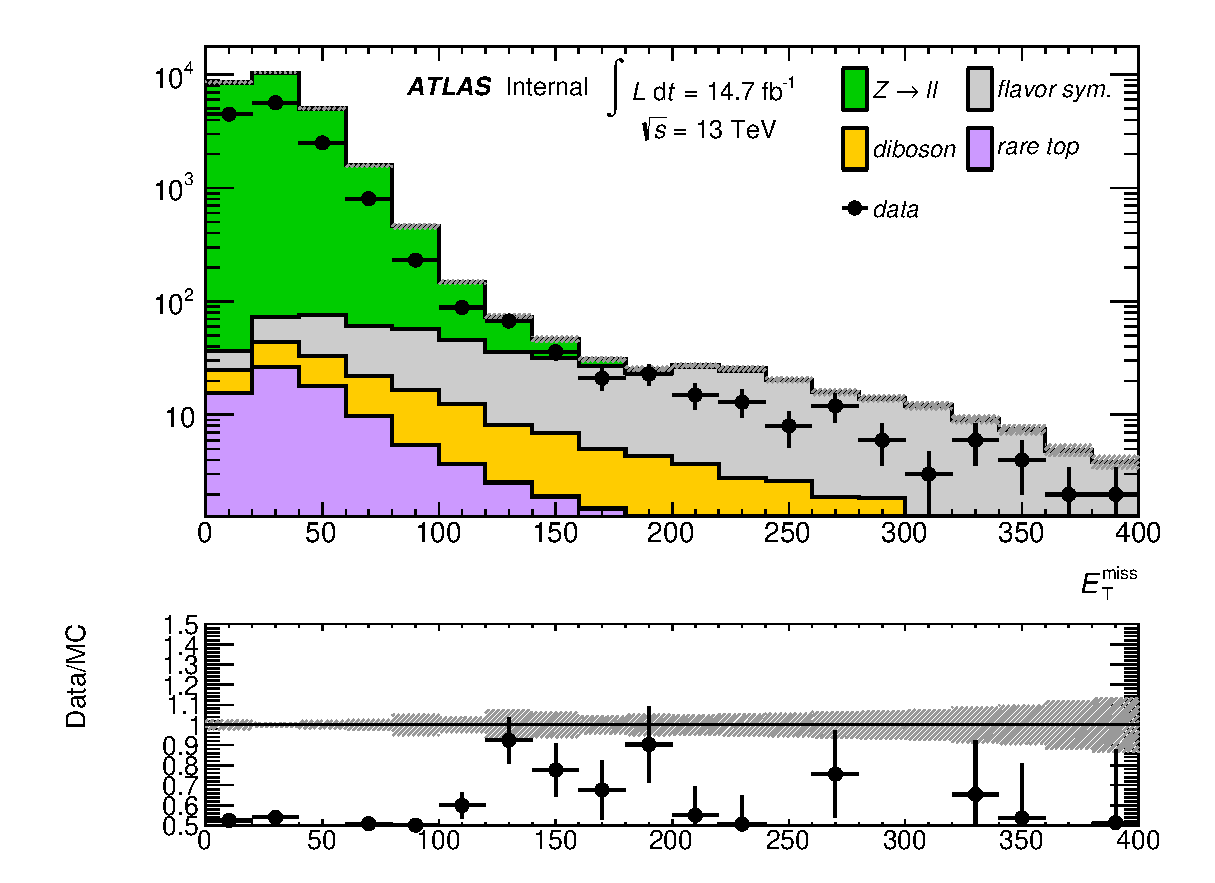
\includegraphics[width=.85\linewidth]{figures/fs/ttbar_met_dependence.eps}
\caption{Comparison of data and \ac{MC} in a selection like SRZ, without the \met cut.}
\label{fig:fs_mc_met}
\end{figure}
\end{centering}

This method is extremely effective as a crosscheck because it uses a completely independent dataset from the flavor symmetry method, and the two methods have very little overlap in dependence on \ac{MC}. They produce consistent results in both SRZ and VRS, as shown in \autoref{tab:fs_comparison}.


\begin{table}[h]
\centering

\begin{tabular}{ccc}
\noalign{\smallskip}\hline\noalign{\smallskip}
Region  & Flavour-symmetry  & Sideband fit  \\
\noalign{\smallskip}\hline\hline\noalign{\smallskip}
SRZ & $33 \pm 4$   &  $29 \pm 7$  \\ [+0.05cm]
VR-S & $99\pm8$        &  $92 \pm 25$  \\ [+0.05cm]
\noalign{\smallskip}\hline\hline
\end{tabular}
\caption{ Comparison of \ac{FS} background predictions from the nominal method, the flavor symmetry method, and the cross-check, the sideband fit method. Uncertainties include statistical and systematic uncertainties in both cases. }
\label{tab:fs_comparison}
\end{table}

%-------------------------------------------------------------------------------------

\section{\dyjets Background}
\label{sec:bg-z}

The \dyjets background is mainly produced by a process called Drell-Yan in which annihilating quark/anti-quark pairs produce a $Z$ boson or a virtual photon. These bosons then decay to two leptons, which, in the case of the $Z$ boson, naturally appear in the $Z$-mass window. The boson typically recoils off a hadronic system, which can satisfy the jet and \HT requirement in SRZ. However, this process rarely produces real \met (though occasionally neutrinos do appear in its hadronic decays), so most events with large amounts of \met are the result of extreme mismeasurement. Because SRZ cuts on the very high \met tails of a $Z$ distribution, a small change in the assumptions about jet resolution or energy scale in \ac{MC} can drastically change the prediction, and a low \dyjets prediction can result in a signal-like peak appearing in the final result. 

Because of this volatility in the \ac{MC} prediction in these high \met tails, a data-driven method is used to estimate this background. The method takes $\gamma$+jets events which, like the \dyjets events, contain one boson recoiling against a hadronic system. These $\gamma$+jets events are then corrected for the kinematic differences between $\gamma$ and $Z$s \cite{ATLAS:2012ema, Chatrchyan:2012qka}. The sample of $\gamma$+jets events is taken from CR-$\gamma$, defined in \autoref{tab:regions-z}. This region is similar to the SRZ selection without the \met requirement, but it vetoes events with leptons and requires at least one photon. Additionally, the $\Delta\phi(\text{jet}_{12},{\boldsymbol p}_{\mathrm{T}}^\mathrm{miss})$ cut in SRZ, which is designed to reduce the background from mismeasured jets, is removed for this region because of its unpredictability at very low values of \met, when the angle of the \met is much less meaningful. 

%TODO what is with the pT miss?

The most significant experimental difference between $Z$ and $\gamma$ events is that $Z$ bosons rapidly decay, in the case of this analysis, to two leptons, which are then be observed by the ATLAS detector. In contrast, the photon is stable, and can be directly detected by ATLAS. This means that the reconstructed $Z$ boson and the directly observed photon have very different energy resolutions.




%-------------------------------------------------------------------------------------

\section{Fake and Non-Prompt Leptons}
\label{sec:bg-fake}

The \textit{fakes} background consists of processes that produce only one lepton, but whose events are otherwise kinematically similar to the \ac{SR}. These processes include semileptonic \ttbar, $W$+jets, and single top processes. Though these processes typically only produce one lepton, they can be reconstructed with two leptons due to a hadron being misidentified as a lepton or due to a real non-prompt lepton resulting from photon conversions or $B$-hadron decays. As such, it includes both events that have been properly reconstructed and many that are included in the \ac{SR} due to imperfect reconstruction. As with the \dyjets background, it is very difficult to predict with \ac{MC} because the flaws in reconstruction are typically less well described by the models used in \ac{MC} production than the successes. Nonetheless, a rough estimate can be made of this background by using \ac{MC}, which indicates that the number of fake events in SRZ is consistent with zero. 

Despite the small predicted contribution in the \ac{SR}, a data-driven method called the \textit{matrix method} is employed to estimate these fake events \cite{SUSY-2013-20}. This method is also used to estimate the fakes contribution to other control and validation regions where their impact is more significant. 

In the matrix method, the quality requirements for signal leptons are loosened to give a selection of baseline leptons (see \autoref{tab:eledef} and \autoref{tab:muondef}), which consist of a higher fraction of fake leptons. In each \ac{CR}, \ac{VR}, or \ac{SR}, the remaining kinematic selections are made on the baseline leptons, and the number of leptons in the region which pass the signal lepton requirements ($N_{pass}$) and the number which fail ($N_{fail}$) are measured. For a 1-lepton selection, these quantities can be used to predict the number of fake events that pass the selection according to:

\begin{equation}
N_{\text{pass}}^{\text{fake}} = \frac{N_{\text{fail}} - (1/\epsilon^{\text{real}} - 1) \times N_{\text{pass}} }{1/\epsilon^{\text{fake}} - 1/\epsilon^{\text{real}}}.
\end{equation}

The efficiencies $\epsilon^\text{real}$ and $\epsilon^\text{fake}$ give the relative identification efficiency from baseline to signal for genuine, prompt leptons and fake and non-prompt leptons, respectively. For a 2-lepton selection, the principle is the same, but the equation is more complicated, requiring a four-by-four matrix to account for possible combinations of real and fake leptons. 


To calculate $\epsilon^\text{real}$, the tag-and-probe method is performed a selection of $Z\rightarrow\ell\ell$ data events, CR-real, described in \autoref{tab:regions-fakes}. In this method, one \textit{tag} lepton passing a signal selection is required, as is another \textit{probe} lepton passing a baseline requirement. Distributions in \mll~for events with a tag and a passing probe and events with a tag and a failing probe are produced and fit, and the efficiency is computed using the ratio acquired from the fit. A comparison of data and \ac{MC} in CR-real can be seen in \autoref{fig:fake_realreg}.
 
\begin{table}[htbp]

\resizebox{1\textwidth}{!}{
 \begin{tabular}{lccccccc} %{\textwidth}{@{\extracolsep{\fill}}lcccccccc}
   \noalign{\smallskip}\hline\noalign{\smallskip}
     {\bf Fakes }   &  {\bf \met}   & {\bf $\HT$}  &  {\bf $n_{\text{jets}}$}  & {\bf $m_{\ell\ell} $} &  {\bf SF/DF}  & {\bf OS/SS} & $n_\ell$\\
     {\bf regions} &  {\bf [\GeV]} & {\bf [\GeV]} &                           & {\bf [\GeV]}          &               &         & \\
   \noalign{\smallskip}\hline\noalign{\smallskip}
   CR-real          &  $-$      &  $\bm{> 200}$  &  $\geq 2$ & {\bf 81--101}    &  $2\ell$ SF  & OS & $2$\\
   CR-fake          &  $\bm{<125}$   &  $-$      &  $-$ & $>12$     &  {\bf $2\ell$ SF/DF}  & {\bf SS} & $\geq2$\\
   \noalign{\smallskip}\hline\noalign{\smallskip}
   \noalign{\smallskip}\hline\noalign{\smallskip}
\end{tabular}
} % end of resizebox
\begin{center}
 \caption{Control regions used to measure efficiencies of real and fake leptons. 
 The flavour combination of the dilepton pair is denoted as either ``SF'' for same-flavour or ``DF'' for different flavour.
The charge combination of the leading lepton pairs are given as ``SS'' for same-sign or ``OS'' for opposite-sign.}
\label{tab:regions-fakes}
\end{center}
\end{table}

\begin{centering}
\begin{figure}[bth]
\myfloatalign
\includegraphics[width=.45\linewidth]{figures/fakes/ee-Cut_Real_TT_HT200-pTsublead_fakes-lin_2016.png}
\includegraphics[width=.45\linewidth]{figures/fakes/mm-Cut_Real_TT_HT200-pTsublead_fakes-lin_2016.png}
\caption{Sub-leading lepton \pT\ for $ee$ (left) and $\mu\mu$ (right) events in the tight-tight region used to measure the real-lepton efficiency for 2016. }
\label{fig:fake_realreg}
\end{figure}
\end{centering}

The fake efficiency, $\epsilon^{fake}$, is determined using the tag-and-probe method in CR-fake, also described in \autoref{tab:regions-fakes}. This region is different from all other regions considered in this analysis because it requires same-sign leptons. Very few processes genuinely produce two same-sign leptons, so this region is enhanced in fake leptons. An upper limit on \met is placed on CR-fake to limit the possible contamination from \ac{BSM} processes. According to \ac{MC}, real, prompt leptons make up about 7\% (11\%) of the baseline electron (muon) sample and about 10\% (61\%) of the signal electron (muon) sample in this region. These real lepton backgrounds are subtracted from the CR-fake yields when calculating the efficiencies. \autoref{fig:fake_fakereg} shows a comparison of data and \ac{MC} in this region.

\begin{centering}
\begin{figure}[htbp]
\centering
\includegraphics[width=.45\textwidth]{figures/fakes/me-Cut_Fake_TT-pTsublead_fakes-lin_2016.png}
\includegraphics[width=.45\textwidth]{figures/fakes/mm-Cut_Fake_TT-pTsublead_fakes-lin_2016.png}
\caption{Sub-leading lepton \pT\ for $\mu e$ (left) and $\mu\mu$ (right) events in the tight-tight region used to measure the fake-lepton efficiency for 2016.}
\label{fig:fake_fakereg}
\end{figure}
\end{centering}

This method is validated in a fakes-rich validation region with a same-sign lepton requirement, \met $\geq$ 50\gev, $\geq$ 2 jets, and a veto on \mll~on the $Z$-mass peak for same flavor channels. The results of this validation can be seen in \autoref{fig:fakes_validation}. With the systematic uncertainties included, the prediction agrees well with the data across a wide range of \mll~values. 

%TODO add this to table

\begin{centering}
\begin{figure}[!htb]
\centering
\includegraphics[width=.45\textwidth]{figures/fakes/ee-CutSSMET_zveto-Mll-lin.pdf}
\includegraphics[width=.45\textwidth]{figures/fakes/mm-CutSSMET_zveto-Mll-lin.pdf}
\includegraphics[width=.45\textwidth]{figures/fakes/em-CutSSMET_zveto-Mll-lin.pdf}
\includegraphics[width=.45\textwidth]{figures/fakes/me-CutSSMET_zveto-Mll-lin.pdf}
\caption{Same sign validation regions in the $ee$ (top left), $\mu\mu$ (top right), $e\mu$ (bottom left) and $\mu e$ (bottom right) channels combining 2015+2016 data. Uncertainty bands include both statistical and systematic uncertainties. \label{fig:fakes_validation}}
\end{figure}
\end{centering}

\section{Diboson and Rare Top Processes}
\label{sec:bg-other}

The remaining backgrounds are diboson processes (excluding $WW$, which is included in the \ac{FS} background) and rare top processes. Dibosons events make up about 30\% of the events in SRZ, while rare top process contributions are much smaller. Both are taken directly from \ac{MC}, with validation regions to confirm the accuracy of the prediction. These regions are described in \autoref{tab:regions-z}, and target different parts of these backgrounds. VR-ZZ is a four-lepton selection designed to select a very pure sample of $ZZ$ events. VR-WZ requires three leptons and makes specific cuts on $m_T$, the transverse mass, and \met in order to select mostly $WZ\rightarrow lll\nu$ events. VR-3L is similar to VR-S, but loosens the \HT and \met cuts and requires at least three leptons. This region is designed to target any $\geq3$-lepton process in a region as kinematically close to SRZ as possible while still maintaining enough events to validate. The makeups of these multilepton validation regions, as well as VRS, are shown in \autoref{tab:VRresults}.



\begin{table}[!htb]
\begin{center}
\setlength{\tabcolsep}{0.0pc}
\resizebox{1\textwidth}{!}{
\begin{tabular*}{\textwidth}{@{\extracolsep{\fill}}lrrrr}
\noalign{\smallskip}\hline\noalign{\smallskip}
                                                                             & VR-S            & VR-WZ        & VR-ZZ          & VR-3L   \\[-0.05cm]
\noalign{\smallskip}\hline\noalign{\smallskip}
Observed events                                                              & $236$            & $698$        & $132$          & $32$ \\
\noalign{\smallskip}\hline\noalign{\smallskip}
%Total expected background events                                             & $223.92 \pm 40.84$   &   $612.97\pm8.65$   &    $139.29\pm4.95$    &    $34.52\pm1.39$ \\
% here the total background uncertainty is updated to the quadrature sum of each bkg uncertainty
Total expected background                                             & $224 \pm 41$   &   $613\pm66$   &    $139\pm25$    &    $35\pm10$ \\
\noalign{\smallskip}\hline\noalign{\smallskip}
  Flavour-symmetric             & $99\pm8$   &   -                &    -                 &    -              \\
  $WZ/ZZ$ events                                                             & $27\pm13$  &   $573\pm66$ &    $139\pm25$        &    $25\pm10$ \\
  Rare top events                                                            & $11\pm3$   &   $14\pm3$   &    $0.44\pm0.11$     &    $9.1\pm2.3$  \\
  \dyjets\ events                                                            & $84\pm37$  &   -                &    -                 &    -              \\
  Fake lepton events                                                         & $4\pm4$    &   $26\pm6$   &    -                 &    $0.6\pm0.3$  \\
 \noalign{\smallskip}\hline\noalign{\smallskip}
\end{tabular*}
} % end of resizebox
\end{center}
\caption{Yields in validation regions. In VRS, data-driven background estimates are used for \dyjets, fakes, and \ac{FS} processes. All other backgrounds are taken from \ac{MC}, including all backgrounds in the multi-lepton \ac{VR}s. Uncertainties include statistical and systematic components. }
\label{tab:VRresults}
\end{table}


To confirm that the kinematics are well modeled in the diboson validation regions, distributions of boson mass and \pt are shown in \ac{MC} and data. Figures \ref{fig:diboson_wz} and \ref{fig:diboson_wz2} show these distributions for VR-WZ, and \autoref{fig:diboson_zz} shows these distributions for VR-ZZ. 

\begin{centering}
\begin{figure}[htbp]
\centering
\includegraphics[width=.9\textwidth]{figures/dibosons/WZ_Wmass.png}
\includegraphics[width=.9\textwidth]{figures/dibosons/WZ_Zmass.png}
\caption{Distribtuions of data and \ac{MC} in VR-WZ. Reconstructed transverse mass of the $W$ (top) and mass of the $Z$ (bottom). \label{fig:diboson_wz}}
\end{figure}
\end{centering}

\begin{centering}
\begin{figure}[htbp]
\centering
\includegraphics[width=.9\textwidth]{figures/dibosons/WZ_Wpt.png}
\includegraphics[width=.9\textwidth]{figures/dibosons/WZ_Zpt.png}
\caption{Distribtuions of data and \ac{MC} in VR-WZ. \pT of the $W$ (top) and $Z$ (bottom). \label{fig:diboson_wz2}}
\end{figure}
\end{centering}

\begin{centering}
\begin{figure}[htbp]
\centering
\includegraphics[width=.9\textwidth]{figures/dibosons/ZZ_Zmass.png}
\includegraphics[width=.9\textwidth]{figures/dibosons/ZZ_Zpt.png}

\caption{Distribtuions in VR-WZ. On the top, mass of the $Z$ bosons in the event, and on the bottom, \pT of the $Z$ bosons. \label{fig:diboson_zz}}
\end{figure}
\end{centering}

